\section{Background and Motivation} \label{sec:motivation}

%In this section, we discuss the key weaknesses of the state-of-the-art function merging, called {\SOAName}~\cite{rocha20}, addressed in this paper.
%First, we show how different stages in {\SOAName} impact its running time.
%\textbf{TODO: Memory usage.}

%In this section, we will discuss how different stages of the state-of-the-art function merging impact during compilation time.
%present how different stages of the state-of-the-art function merging impact its running time.
%In this section, we will present how sequence alignment can be an important source of compilation time overhead.
%Then we discuss how we can address this issue by doing less work, while still keeping most of the code size reduction from the state-of-the-art technique.

In this section, we first provide an overview of the working mechanism of \SOAName, described in Chapter~\ref{chp:pldi20}. We highlight the main drawbacks of \SOAName in terms of compile time and memory footprint. We then outline how we can address these drawbacks without compromising on code size reduction. 

\subsection{Function Merging via Sequence Alignment}
Existing function merging techniques consist of three major stages: choosing which functions to merge, producing the merged function, and estimating the merging profitability.
%\fixme{PP: Is it accurate to talk about two major stages in SalSSA and also this being the case for most optimizations?}

In order to pair similar functions for merging, \SOAName employs a ranking strategy based on the similarity of the \textit{fingerprints} of the functions.
A fingerprint summarizes the content of a function as a fixed-size vector of the frequency of each LLVM-IR opcode. The representation allows the compiler to compare functions using a simple distance metric, such as the Manhattan distance. For a given reference function, all other functions are ranked based on their distance and the closest function is chosen for merging.

Merging two functions requires identifying similar code segments in the two functions that can be profitably merged.
The main innovation of \SOAName~\cite{rocha20} and its predecessor~\cite{rocha19} is the use of a sequence alignment algorithm, called the \NW algorithm, for identifying similar code segments.
This allows them to merge arbitrary pairs of functions.
First, they transform each function into a linear sequence of labels and instructions.
Then, the alignment algorithm is applied on the sequences of the whole input functions.
The resulting alignment is used to generate the merged function.
Once the merged function has been generated, they apply an SSA reconstruction algorithm.
For a final clean up, they simplify the merged function by removing redundant instructions introduced by function merging.
% PP: still not sure that this information is useful for understanding our contribution

Finally, a profitability analysis estimates the benefit of replacing the original pair of functions with the simplified merged function. If unprofitable, the merged function is simply thrown away. Otherwise, they delete the original functions, redirecting the calls to the merged function.
%If the original functions cannot be deleted, e.g., because they might be called externally, their body is replaced by a call to the merged function.
% PP: Similarly not really important for understanding our contribution

\subsection{Limitations of The State of The Art}
%PP: I think we should reorganise this a bit. After refocusing the discussion here on memory, jumping to a subsection called "Compilation Overhead Breakdown" that mainly talks about compilation time seems disconnected. Instead, we should merge the two subsection making the first half about the limitations in terms of memory and the second about the limitations in terms of runtime.

When reproducing the {\SOAName} experiments using the available artifact~\cite{rocha20} on our machine, we were unable to build \texttt{602.gcc\_s}, from SPEC 2017, due to an out of memory crash. 16~GB of memory were not enough for {\SOAName}. 
We succeeded only after migrating to a 64~GB machine which could fit the 32~GB of temporary data produced by function merging.
After investigating further, we realized that this is due to the quadratic algorithm used for aligning the two functions selected for merging.
Because this algorithm is applied on the linearized sequences of the whole input functions, \SOAName incurs a high memory footprint when merging even medium sized functions.
For larger ones, it is impossible to apply it on most workstations or even many servers, making {\SOAName} impractical for use in production.
%For the same reason, alignment brings the compilation process to a crawl for large functions.


%\subsection{Compilation Overhead Breakdown}
\label{sec:motivation:breakdown}

%When merging two functions, the goal is to identify which segments of the code are different and which ones are equivalent, and therefore mergeable.
%To this end, SalSSA uses an optimal sequence alignment algorithm, called the Needleman-Wunsch algorithm, which is quadratic on the size of the input sequences.
%Since SalSSA applies it on the linearised sequences of the whole input functions, the time spend aligning sequences can be significant for programs with very large functions.

For the same reason, alignment brings the compilation process to a crawl for large functions.
Figure~\ref{fig:compilation-breakdown-motivation-alignment} shows the running time breakdown for the different stages of the function merging pass in the LLVM-based \SOAName  implementation for two SPEC CPU2017 benchmarks. 
Sequence alignment dominates the running time of function merging, representing up to 83\% of its overall running time. 
Sequence alignment alone takes 25 seconds and 4.2 minutes on \texttt{638.imagick\_s} and \texttt{602.gcc\_s}, respectively.
%PP: Remove the next sentence?
The alignment stage also causes the peak in memory usage for these two programs, 4.5~GB for \texttt{638.imagick\_s} and 32~GB for \texttt{602.gcc\_s}.
This is not surprising, as the Needleman-Wunsch algorithm has a quadratic complexity in both time and memory usage.
Because this algorithm is applied on linearized sequences of the whole input functions, programs containing large functions, such as the ones in our example, are heavily affected.
%For example, \texttt{638.imagick\_s} has a total of 15,454 functions with the largest one having 73,127 instructions.
%Meanwhile, even though \texttt{602.gcc\_s} has only 2,457 functions, its largest function has 28,974 instructions; hence \SOAName also incurs significant peak memory usage when processing this program. 

\begin{figure}[h]
  \centering
  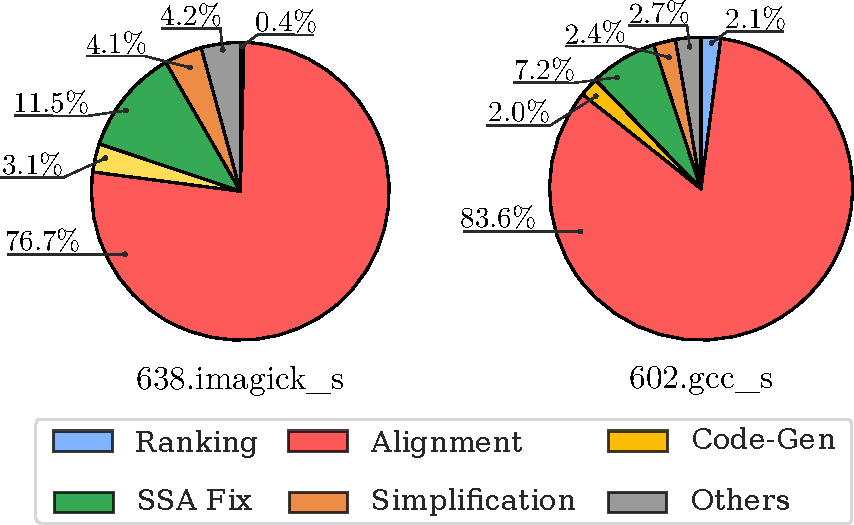
\includegraphics[width=0.7\linewidth]{src/lctes21/figs/compilation-breakdown-motivation-alignment.pdf}
  \caption{Breakdown of the relative runtime for the different stages from {\SOAName}. Alignment takes 25 seconds and 4.2 minutes on \texttt{638.imagick\_s} and \texttt{602.gcc\_s}, respectively.}
  \label{fig:compilation-breakdown-motivation-alignment}
\end{figure}

Most of the rest of the running time of function merging is associated with producing merged functions from the aligned sequences.
%\fixme{PP: Same suggestion as earlier about CodeGen.}
This includes the time spent on the code generation stage (Code-Gen), SSA reconstruction (SSA Fix), and code simplification (Simplification). These stages account for 18.7\% of the {\SOAName}’s running time on \texttt{638.imagick\_s} and 11.6\% on \texttt{602.gcc\_s}.
However, for other programs, these stages may represent the vast majority of {\SOAName}’s running time (see Section~\ref{sec:eval:pass-speedup}).

This breakdown includes the cost for producing both \emph{profitable} and \emph{unprofitable} merged functions.
In fact, most of it is wasted on merged functions that will be rejected by the profitability analysis.
These costs are pronounced because unprofitably merged functions have no limit on their size or complexity, often adding a significant pressure on the SSA reconstruction and simplification stages.
This effect is tied to the alignment strategy, since a good alignment is needed for producing profitably merged functions.
As we discuss in Section~\ref{sec:motivation:less-more}, a better approach would include a finer grain profitability analysis that would allows us to bail out from merging complex and unprofitable code as early as possible.

\subsection{When Less is More} \label{sec:motivation:less-more}

We observe that most of the benefit of function merging often comes from merging highly similar, but not necessarily identical, basic blocks. Figure~\ref{fig:xalan-example} shows one such example extracted from the \texttt{483.xalancbmk} benchmark found in SPEC CPU2006.
This example shows the two input functions annotated with the alignment produced by \SOAName. Merging these two functions contributes to a reduction of 33 bytes in the final object file.

\begin{figure}[h]
  \centering
  \includegraphics[width=\linewidth]{src/lctes21/figs/xalan-example.pdf}
  \caption{Example extracted from \texttt{483.xalancbmk} in SPEC CPU2006. Instructions marked green have been aligned through sequence alignment with an instruction from the other function. {\SOAName} would attempt merging all matched instructions but only the ones in fully aligned basic blocks would be profitable.}
  \label{fig:xalan-example}
\end{figure}

% \begin{figure*}[h]
%   \centering
%   \includegraphics[width=0.6\textwidth]{figs/xalan-example.pdf}
%   \caption{Example extracted from \texttt{483.xalancbmk} found in SPEC CPU2006.}
%   \label{fig:xalan-example}
% \end{figure*}

%This example also suggests that 
While this approach is flexible enough to identify very complex alignments, what it actually produces is three aligned pairs of basic blocks and a few aligned instructions in the entry blocks. More importantly, these entry block instructions offer nothing in terms of code size reduction. The gains of merging them are negated by the extra branches and operand selections needed to preserve the program's semantics. Since {\SOAName} analyzes the profitability of the final merged function as a whole, this unprofitable sequence of instructions will be merged because of the three highly profitable basic blocks. For the same reason, we may have profitable areas of code rejected because the rest of the merged function is unprofitable.


%Since {\SOAName} analyzes the profitability of the final merged function as a whole, we may have segments of unprofitably merged code inside an otherwise profitably merged function.
%Similarly, we may also have segments of profitably merged code inside merged functions that are thrown away by the profitability analysis. 
%However, we can achieve the same code size reduction of 33 bytes by merging only the subset of nearly identical basic blocks (highlighted in Figure~\ref{fig:xalan-example}).
%The gains of merging the entry blocks are negated by the extra branches and operand selections needed to preserve the program's semantics.

This example shows us that we could achieve similar code size reduction by breaking the problem of aligning functions into two simpler processes: first identifying highly similar basic blocks and then aligning the instructions in each pair of similar blocks. 
%merging functions on the basic block rather than on the instruction level adopted by \SOAName.
By operating on basic blocks, we could greatly reduce the length of the sequences to be aligned and the associated compilation and memory overhead. Furthermore, by making profitability decisions for each pair of basic blocks separately, we could avoid merging unprofitable pairs. The rest of this chapter shows how we use such an approach to overcome the weaknesses of \SOAName and make function merging practical for optimizing large programs. 

%Therefore, the main takeaways are:
%1) It often suffices to merge functions on a per basic block manner. %, since crossing the basic block boundary is rarely necessary.
%2) A fine-grain profitability analysis is needed to avoid  merging unprofitable pairs of basic blocks.



%This happens because the optimal sequence alignment algorithm used by SalSSA is trying to maximize the number of matching entries, which does not necessarily translate to the optimal merged function.
%Moreover, SalSSA is also limited by the fixed linearization strategy.
%For example, the two \textit{return} instructions are not aligned due to the ordering of the basic blocks chosen by the linearization strategy.

%We can take advantage of this insight in order to design a faster function merging technique.
%Ultimately, our goal is to be able to avoid the quadratic algorithm while still producing significant reductions to the program's size.

%In this paper, we take advantage of these key insights to propose a novel function merging technique that addresses the major overheads discussed in Section~\ref{sec:motivation:breakdown}.
%We can take advantage of this insight in order to design a better and faster function merging technique.
%To this end, we propose a novel function merging technique that work on the level of basic blocks and includes a fine-grain profitability analysis.



%bail out early from   of a fine-grain and a coarse-grain analysis.

%TODO: [Relatedwork] Note that this is different from the work done by von Koch~et~al.~\cite{edler14}, as these two functions are not \textit{structurally similar} as expected by their function merging technique and therefore could not be merged.
